\section{Motivation for Higgs Pair Production}

% Super excellent talk by Katharine:
% https://indico.cern.ch/event/1065153/attachments/2351166/4011032/Seminar.pdf

Taylor expansion of the Higgs potential about the minimum after EWSB:
\begin{align*}
  V(h) &= \frac{1}{2} m_{\PH}^2 h^2 + \lambda v h^3 + \frac{1}{4} \lambda h^4 + \dots \\
  m_{\PH} &= \sqrt{2 \lambda v} \approx \SI{125}{\GeV} \\
  \lambda &\approx 0.13 \quad \text{(SM)}
\end{align*}
$h$ is a complex field with the $h^2$-term being the mass term,
$h^3$-term yielding the trilinear coupling, and the $h^4$-term
yielding the quartic coupling. All these terms are directly predicted
by the SM but an experimental probe is still justified to detect
possible deviations from the SM. The self-coupling strength~$\lambda$
can be directly probed in either double Higgs boson production or
triple Higgs boson production (although inaccessible
currently). Indirect probes also exist for example in single Higgs
boson production where the self-coupling contributes at loop-level.

Cross section of HH production is 1000 times smaller than single
Higgs. \todo{Cross section diagram would be nice?}

Motivation:
\begin{description}

\item[Vacuum Stability] The present minimum with a vacuum expectation
  value of $v \approx \si{246}{\GeV}$ might be either a global minimum
  in which case the universe is stable or only a local minimum which
  leads to a metastable universe. In the metastable case, the state of
  the Higgs field could tunnel to a new local or global minimum with a
  smaller vacuum expectation value. Current experimental data cannot
  distinguish whether the universe is stable or
  meta-stable\todo{citation}.

\item[Elektroweak phase transition] In baryogenesis a first order
  electroweak phase transition is needed.

\item[BSM] Radions, 2HDM, Warped extra dimensions, composite Higgs,
  hMSSM, KK Gravitons: Most could decay to pairs of SM Higgs bosons.

\end{description}



\subsection{Search channels for Higgs boson pair production}

\begin{figure}[htbp]
  \centering
  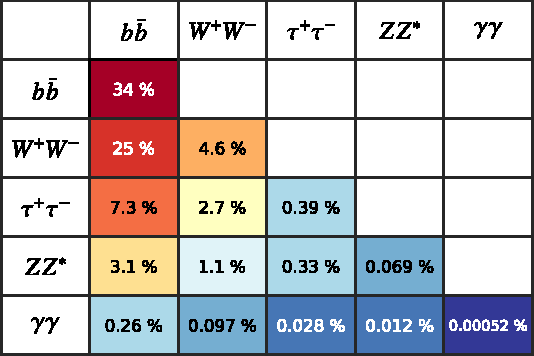
\includegraphics[width=0.45\textwidth]{theory/di_higgs_branching_ratio}
  \caption{Possible final states of decays of pairs of Standard Model
    Higgs bosons. Higgs boson branching ratios are taken
    from~\cite{deFlorian:2016spz} and
    assume~$m_{\PH} = \SI{125.0}{\GeV}$. The decay
    mode~$\PH \ra \Pgluon\Pgluon$ is neglected due to limited
    experimental feasibility.}
  \label{fig:hh_branching_ratios}
\end{figure}

4b: Very large branching ratio but huge multi-jet background.

bbtautau: Can suppress multi-jet background reasonably but large
backgrounds from EW and top.

bbyy: Very clean, but low BR.



Sensitivity vs mass:

bbyy: Low mass sensitivity (due to low threshold photon triggers)

bbtautau: Medium mass sensitivity

bbbb: High mass sensitivity (BR and reduced problems in finding Higgs
candidates due to boost)


\subsection{Review of searches for Higgs boson pair production}

Brief review of previous results / prospects.



%%% Local Variables:
%%% mode: latex
%%% TeX-master: "../../phd_thesis"
%%% End:
